%%%%%%%%%%%%%%%%%%%%%%%%%%%%%%%%%%%%%%%%%%%%%%%%%%%%%%%%%%%%
% % Title and the authors % %
%%%%%%%%%%%%%%%%%%%%%%%%%%%%%%%%%%%%%%%%%%%%%%%%%%%%%%%%%%%%
\title{Morse Theory}
\author{ Miloš Vukadinović \\ Veronika Starodub \\ Nikolay Ninov} \date{\today } 

\documentclass[]{article}
\usepackage{graphicx}

\usepackage[utf8]{inputenc}
\usepackage{setspace}
\usepackage{amsthm}
\usepackage{amssymb}
\usepackage{amsmath}
\usepackage{hyperref}
\usepackage{tikz}
\usetikzlibrary{matrix}

\newtheorem{theorem}{Theorem}
\newtheorem{lemma}{Lemma}
\newtheorem{example}{Example}
\newtheorem{problem}{Problem}
\newtheorem{proposition}{Proposition}
\newtheorem{scolium}{Scolium} 
\newtheorem{definition}{Definition}

\newcommand{\R}{\mathbb{R}}
\newcommand{\Z}{\mathbb{Z}}
\newcommand{\X}{\mathbb{X}}
\newcommand{\imply}{\Rightarrow}

\graphicspath{{images/}} 

% \doublespacing
\begin{document} 
\maketitle

\begin{figure}[h]
    \centering
    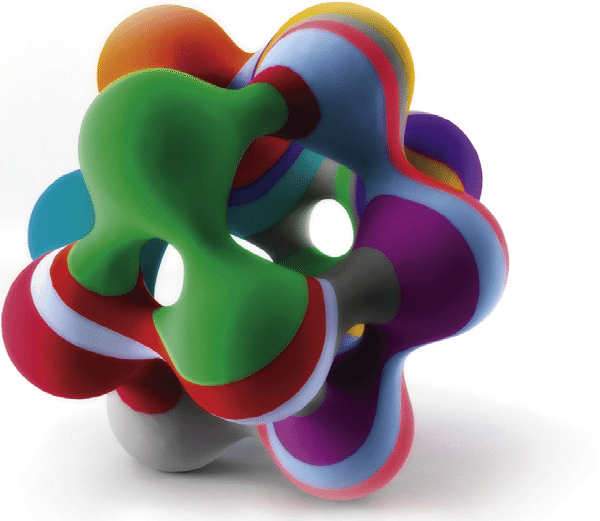
\includegraphics[width=0.50\textwidth]{cover}
\end{figure}
 
\tableofcontents
\newpage
A smooth function is always good to have. However, some critical points might have equal function values. Morse functions are such ones that don't have the latter property. 
Sometimes we would like to analyze a function, using its level sets. A Reeb graph helps us plot the evolution of the components of a level set. Morse functions and Reeb graphs are extremely useful
in some contexts. They have applications in topological data analysis, computer graphics, and even in oceanography.
\section{Morse Theory}
%%%%%%%%%%%%%%%%%%%%%%%%%%%%%%%%%%%%%%%%%%%%%%%%%%%%%%%%%%%%%%%%%%%%%%%%%%%%%%%%%%%%%
% % begin N1
\subsection{Introduction}

\begin{definition}(Morse function)
A smooth function on a manifold is a Morse function if 
\begin{itemize}
	\item all critical points are non-degenerate
	\item the critical points have distinct function values
\end{itemize}
\end{definition}

\begin{theorem}
        Let $f$ be a smooth function in a neighborhood 
    $N_x$ of $x=(x_1,\ldots,x_n)$ in $\mathbb{R}^n$. Suppose $f(0,\ldots,0)=0$. Then, 
    there exist $n$ smooth functions $g_i,\ldots,g_n$ defined on $N_x$ such that $g_i(0,\ldots,0)=\frac{\partial f}{\partial x_i}(0,\ldots,0)$
    for every $i$, and

    $$
        f(x_i,\ldots,x_n)=\sum_{i=1}^{n}{(x_i,\ldots,x_n)}
    $$
\end{theorem}
\begin{theorem}(Inverse Function Theorem)
        Let $f:\mathbb{R}^n\to \mathbb{R}^n$ be a smooth function on an open set $U$
        containing $a\in\mathbb{R}^n$. Suppose that $\det J_f(a)\not = 0$.
        \\Then there is an open set $V \subset \mathbb{R}^n$ containing $a$ and an open
        set $W\subset \mathbb{R}^n$ containing $f(a)$ such that $f:V\to W$ is a 
        diffeomorphism. 
\end{theorem}
\begin{theorem}(Morse Lemma.)
        Suppose that the point $a \in \mathbb{R}^k$ is a nondegenerate
        critical point of the function $f$, and
        $$
            (h_{ij})= \left(  \frac{\partial^2f}{\partial x_i \partial x_j} (a) \right)
        $$
        is the Hessian of $f$ at $a$. Then there exists a local coordinate system $(x_1,\ldots,x_k)$ around $a$ such that
        $$
            f=f(a)+\sum{h_{ij}x_ix_j}
        $$
        near $a$.
        \\
        or
        $$
            f=-x_1^2-x_2^2-\ldots-x_\lambda^2+x_\lambda^2+\ldots+x_n^2+f(a)
        $$
        where $\lambda$ is the index of $f$ at $a$.
\end{theorem}
\begin{proof}
     Let $p_0$ be a nondegenerate critical point of the function
     $f:\ M \to \mathbb{R}$, where $M$ is an $n$-manifold. The degeneracy of the point
     $p_0$ on $f$ is determined independent of our choice of a local coordinate system.
     Therefore, we may assume that when we pick a local coordinate system $(x_1,\ldots,x_n)$ defined
     in a neighborhood $N_{p_0}$,

     \begin{equation}
        \frac{\partial^2f}{\partial x_1^2}(p_0)\not = 0\tag{1.1}
     \end{equation}

    or that we may pick a suitable linear transformation of the local coordinate
    system such that equation $1.1$ is true. We may further assume that $p_0$ corresponds
    to the origin $(0,\ldots,0)\in \mathbb{R}^n$ on the local coordinate system and that $f(p_0)=0$,
    replacing $f$ with $f-f(p_0)$ if necessary.
    
    By Theorem 1.1, there exit $n$ smooth functions $g_i,\ldots,g_n$ defined on
    $N_{p_0}$ such that

     \begin{equation}
        g_i(0,\ldots,0)=\frac{\partial f}{\partial x_i}(0,\ldots,0) \tag{1.2}
     \end{equation}

     and

     \begin{equation}
        f(x_1,\ldots,x_n)=\sum_{i=1}^{n}{(x_1,\ldots,x_n)}\tag{1.3} 
     \end{equation}

     But since $p_0$ is a critical point, equation $1.2$ turns out to be zero on both 
     sides at $p_0$. So we can apply Theorem $1.1$ again to get $n$ smooth functions 
     $h_{i1},\ldots,h_{in}$ for every $i$ that is defined on $N_{p_0}$ such that

     \begin{equation}
        \sum_{j=1}^{n}{x_jh_{ij}(x_1,\ldots,x_n)}=g_i(x_1,\ldots,x_n) \tag{1.4}
     \end{equation}

     By plugging equation $1.4$ into equation $1.3$, we get

     \begin{equation}
        f(x_1,\ldots,x_n)=\sum_{i=1}^{n}\sum_{j=1}^{n}{x_ix_jh_{ij}(x_1,\ldots,x_n)} \tag{1.5}
     \end{equation}

     We may assume that $h_{ij}=h_{ji}$, rewriting $h_{ij}$ as
     $H_{ij}=\frac{h_{ij}+h_{ji}}{2}$ if necessary. Furthermore,

     \begin{equation}
        (h_{ij}(0,\ldots,0))_{n \times n}=\left( \frac{1}{2}\frac{\partial^2f}{\partial x_i \partial x_j}(0,\ldots,0)_{n\times n} \right) \tag{1.6}
     \end{equation} 
     And since we assumed equation $1.1$ to be true, then $h_{11}(0,\ldots,0)\not = 0$. $h_{11}$
     is a smooth, hence continuous function, and so $h_{11}$ is not zero in a neighborhood of the origin.
     Let us call this neighborhood $\bar{N}_0$    

     Our ultimate goal is to express $f$ in the standard quadratic form of the equation from the lemma.
     We do this by eliminating all terms which are not of the form $\pm x_i^2$ via induction over $k\le n$
     steps. While we are currently dealing with $k=1$, in the general case of $k$, we wish to express $f$ 
     as a sum of terms such that $k$ terms are of the form $\pm x_i^2$ and the rest of the terms depend
     on coordinate in the set ${x_i|i\not = k}$. To this end, let
     \begin{equation}
        G(x_1,\ldots,x_n)=\sqrt{|h_{11}(x_1,\ldots,x_n) | }   \tag{1.6}
     \end{equation}
        
     G is a smooth, non-zero function of $x_1,\ldots,x_n$ on $\bar{N}_0$.

     Now suppose by induction that there exists a local coordinate system $(y_1,\ldots,y_n)$ defined on $\bar{N}_0$ such that
     \begin{equation}
        y_i=x_i(\not = 1) \tag{1.7}
     \end{equation}
     \begin{equation}
        y_1=G*(x_1+\sum_{i>1}^{n}{\frac{x_ih_{1i}}{h_{11}}})\tag{1.8}
     \end{equation}

     It follows from the Inverse Function Theorem that $y_1,\ldots,y_n$ is a local
     coordinate system defined on a smaller neighborhood $\tilde{N}_0 \subset \bar{N}_0$,
     since the determinant of the Jacobian of the transformation from $(x_1, \ldots,x_n)$
     to $(y_1,\ldots,y_m)$ may be verified to be nonzero.

     When we square $y_1$, we get
     \begin{equation}
        y_1^2=\pm h_{11}x_1^2\pm2\sum_{i=2}^{n}{x_1x_ih_{1i}}\pm\frac{\left(\sum_{i=2}^{n}{x_ih_{1i}}\right)^2}{h_{11}}\tag{1.9}
     \end{equation}
     where the signs are either positive or negative, depending on the sign of $h_{11}$. Using equation
     $1.5$, we can verify that $f$ can be expressed in the following way with respect to this
     coordinate system on the restricted domain $\tilde{N}_0$.
     \begin{equation}
        f=\pm y_1^2 + \sum_{i=2}^{n}\sum_{j=2}^{n}{x_ix_jh_{ij}}-\frac{\left(\sum_{i=2}^{n}{x_ih_{1i}}\right)^2}{h_{11}}\tag{1.10}
     \end{equation}
     where the sign of the $y_1^2$ term is positive or negative, depending on the sign of $h_{11}$. Staying
     consistent with our goals, we notice that the first term is in the standard quadratic form seen
     in the Morse Lemma formulation, whereas the rest of the terms depend on local coordinates
     $x_i$ whereby $i\not=k \ (k=1)$. By induction from $k=1$ to $k=n$, we prove the Morse Lemma.
\end{proof}
% % end N1
%%%%%%%%%%%%%%%%%%%%%%%%%%%%%%%%%%%%%%%%%%%%%%%%%%%%%%%%%%%%%%%%%%%%%%%%%%%%%%%%%%%%%%%%%%%%%%%%%%%%%%%%%%%%%%
%%%%%%%%%%%%%%%%%%%%%%%%%%%%%%%%%%%%%%%%%%%%%%%%%%%%%%%%%%%%%%%%%%%%%%%%%%%%%%%%%%%%%%%%%%%%%%%%%%%%%%%%%%%%%%
% % begin M1

\subsection{Examples of Morse functions} 
\begin{problem}
Show that the function $f: S^2 \to \R, f(x,y,z) = z$ is a Morse function.
\end{problem}
$f$ is smooth on $ S^2 $ since it extends to a smooth map on all of $\R^3$. We can map $R^3$ to $S^2$ with the stereographic projection two functions:
\begin{equation}
	\phi_1(x_1,x_2,x_3) = (\frac{x_1}{1-x_3}, \frac{x_2}{1-x_3} ) 
\end{equation}
and
\begin{equation}
	\phi_2(y_1,y_2,y_3) = (\frac{y_1}{1+y_3},\frac{y_2}{1+y_3})
\end{equation}
Therefore, to get $S^2 \to R^3$ we can take $\phi_1^{-1}$ and $\phi_2^{-1}$ \\
\begin{equation}
\phi_1^{-1}(x_1,x_2,x_3) = (\frac{2x_1}{x_1^2+x_2^2+1}, \frac{2x_2}{x_1^2+x_2^2+1}, \frac{x_1^2+x_2^2-1}{x_1^2+x_2^2+1})
\end{equation}
\begin{equation}
	\phi_2^{-1}(y_1,y_2,y_3) = (\frac{2y_1}{y_1^2+y_2^2+1}, \frac{2y_2}{y_1^2+y_2^2+1}, \frac{1-y_1^2+y_2^2}{y_1^2+y_2^2+1})
\end{equation}
Then, we take $g_1 = f \circ \phi_1^{-1}$ and $g_2 = f \circ \phi_2^{-1}$ \\
\begin{equation}
	g_1(x,y) =  \frac{x^2+y^2-1}{x^2+y^2+1}
\end{equation}
and
\begin{equation}
	g_2(x,y) = \frac{1-x^2+y^2}{x^2+y^2+1}
\end{equation}
Now, we can compute jacobian of $g_1$ and $g_2$, find critical points, and check that determinant of hessian matrix is non-zero. \\
$
	\nabla g_1(x,y,z) = 0$ iff $(x,y,z) = (0,0,-1)
$\\
$
	\nabla g_2(x,y,z) = 0$ iff $ (x,y,z) = (0,0,1)
$
We have two critical points, and now we compute the hessian at them.\\

\begin{equation}
	H(g_1) = \begin{bmatrix} 4 & 0 \\ 0 & 4 \end{bmatrix}
	\imply \det(H(g_1)) = 16
\end{equation}
\begin{equation}
	H(g_2) = \begin{bmatrix} -4 & 0 \\ 0 & -4 \end{bmatrix}
	\imply \det(H(g_2)) =  16
\end{equation}
Both critical points are non-degenerate, therefore $f$ is a Morse function.$\blacksquare$\\
% % end M1
%%%%%%%%%%%%%%%%%%%%%%%%%%%%%%%%%%%%%%%%%%%%%%%%%%%%%%%%%%%%%%%%%%%%%%%%%%%%%%%%%%%%%%%%%%%%%%%%%%%%%%%%%%%
%%%%%%%%%%%%%%%%%%%%%%%%%%%%%%%%%%%%%%%%%%%%%%%%%%%%%%%%%%%%%%%%%%%%%%%%%%%%%%%%%%%%%%%%%%%%%%%%%%%%%%%%%%%
% % start V1
\\
\\
\begin{example}
$f(x,y)=e^{xy}+x$ is a Morse function
\end{example}
First of all we have to find all critical points of $f$. A point $P$ is critical, when $\frac{\partial f}{\partial x}=\frac{\partial f}{\partial y}=0$ at $P$. \\
$\frac{\partial f}{\partial x}= ye^{xy}+1=0 \\
\frac{\partial f}{\partial y}=xe^{xy}=0$
After solving the system of equations we get that $x=0$, $y=-1$. Hence, the only critical point of $f$ is $(0,-1)$. Now to prove that the function is a Morse function we have to shoe that the determinant of Hessian matrix at the point $(0,-1)$ is non-zero. \\
Partial second order derivatives are: \\
$\frac{\partial^2 f}{\partial x^2}=y^2e^{xy}$
$\frac{\partial^2 f}{\partial x^2}(0,-1)=1$\\
$\frac{\partial^2 f}{\partial \partial y}=e^{xy}+yxe^{xy}$
$\frac{\partial^2 f}{\partial \partial y}(0,-1)=1$\\
$\frac{\partial^2 f}{\partial y \partial x}=e^{xy}+xye^{xy}$
$\frac{\partial^2 f}{\partial y \partial x}(0,-1)=1$\\
$\frac{\partial^2 f}{\partial y^2}=x^2e^{xy}$
$\frac{\partial^2 f}{\partial y^2}(0,-1)=0$\\
Therefore, \\
$det(Hess(f(0,-1)))=\left| \begin{array}{cc} 1 & 1 \\ 1 & 0 \end{array} \right|=-1$. \\
Since the determinant is non-zero at the only critical point of the function, we can claim that it is a Morse function. \\
\begin{example}
Let's consider a function $g(x,y)=xy$ and prove that it is , indeed, a Morse function.\\ 

\end{example}
First order partial derivatives: \\
$\frac{\partial g}{\partial x}=y$\\
$\frac{\partial g}{\partial y}=x$\\
Therefore, the only critical point of $g$ is $(0,0)$. Now we have to evaluate the determinant of Hessian matrix at this point.\\
Second order partial derivatives: \\
$\frac{\partial^2 g}{\partial x^2}=0$\\
$\frac{\partial^2 g}{\partial x \partial y}=1$\\
$\frac{\partial^2 g}{\partial y \partial x}=0$\\
$\frac{\partial^2 g}{\partial^2 y}=1$\\
Hence the determinant of Hessian at the critical point is: \\
$det(Hess(f(0,0)))=\left| \begin{array}{cc} 0 & 1 \\ 1 & 0 \end{array} \right|=-1$. \\
We observe that the determinant is nonzero, hence, the only critical point of $g(x,y)=xy$ is non-degenerate, so the function is Morse. \\
\\
\\
\subsection{Examples of non-Morse functions} 
\begin{example}
$f(x,y)=x^3+xY^2-x^2y-y^3$
\end{example}
Let's follow the previous procedure: \\
$\frac{\partial f}{\partial x}=3x^2+y^2-2xy=0$\\
$\frac{\partial f}{\partial y}=2xy-x^2-3y^2=0$\\
After solving the system of equations we got that the only critical point of $f$ is $(0,0)$. Now compute second order partial derivatives:\\
$\frac{\partial^2 f}{\partial x^2}=6x-2y$\\
$\frac{\partial^2 f}{\partial x \partial y}=2y-2x$\\
$\frac{\partial^2 f}{\partial y \partial x}=2y-2x$\\
$\frac{\partial^2 f}{\partial^2 y}=2x-6y$\\
Therefore, \\
$det(Hess(f(0,0)))=\left| \begin{array}{cc} 0 & 0 \\ 0 & 0 \end{array} \right|=0$.\\
Hence, the only critical point of $f$ is degenerate, so $f$ is not a Morse function. \\
$g(x,y)=x^3$\\
$\frac{\partial g}{\partial x}=3x^2$\\
$\frac{\partial g}{\partial y}=0$\\
Therefore, critical points are all points of the form $(0, y_1)$.\\
$\frac{\partial^2 g}{\partial x^2}=6x$
$\frac{\partial^2 g}{\partial x \partial y}=0$\\
$\frac{\partial^2 g}{\partial y \partial x}=0$
$\frac{\partial^2 g}{\partial^2 y}=0$\\
Hence, Hessian will be of the form: \\
$Hess(g(0,y_1))=\left| \begin{array}{cc} 0 & 0 \\ 0 & 0 \end{array} \right|,  \forall y_1$. \\
Therefore, all critical points of $g$ are degenerate points, moreover, values of $g$ at all critical points are equal, hence, $g(x,y)=x^3$ is not a Morse function. 
% % end V1
%%%%%%%%%%%%%%%%%%%%%%%%%%%%%%%%%%%%%%%%%%%%%%%%%%%%%%%%%%%%%%%%%%%%%%%%%%%%%%%%%%%%%%%%%%%%%%%%%%%%%%%%%%%%%%%%%%%%%%%%%%%%%%%%%%%%%%%%%%%%%%%%%%%%%%%%%%%%%%%%%%%
\newpage
\section{Reeb graphs}
     \subsection{Introduction to Reeb graphs}
     \paragraph{}
      Suppose we have an equivalence relation, $\sim$, defined on a topological space $\X$. Let $\X_\sim$
      be the set of equivalence classes and let $\phi : \X \to \X_\sim$ map each point $x$ to its equivalence class.

\begin{definition}
      Let $f: \X \to \R$ be continuous and call a component of a level set a contour. Two
      points $x,y \in \X$ are equivalent if they belong to the same component of $f^{-1}(t)$
      with $t=f(x)=f(y)$. The Reeb graph of $f$, denoted as $R(f)=\X_\sim$, is the quotient space 
      defined by this equivalence relation.
  \end{definition}
      By construction, the Reeb graph has a point for each contour and the connection is 
      provided by the map $\phi:\X\to R(f)$. Letting $\pi:R(f)\to\R$ be defined such that $f(x)=\pi(\phi(x))$
      we can construct the level set by going backward, from the real line to the Reeb graph to the 
      topological space. Given $t\in\R$ we get $\pi^{-1}(t)$, a collection of points in $R(f)$,
      and $\phi^{-1}(\pi^{-1}(t))$, the corresponding collection of contours that make up the level set defined by $t$.

      \paragraph{Notes:}We have a continuous surjection $\phi:\X\to R(f)$ which maps components 
      to components. Furthermore, a loop in $\X$ that maps to a loop in $R(f)$ is not contractible
      and two loops in $\X$ that map to different loops in $R(f)$ are not homologous. It follows
      that the number of components is preserved and the number of loops cannot increase:
      $$
      \beta_0(R(f))=\beta_0(\X)
      $$
      $$
      \beta_1(R(f))\le\beta_1(\X)
      $$

%%%%%%%%%%%%%%%%%%%%%%%%%%%%%%%%%%%%%%%%%%%%%%%%%%%%%%%%%%%%%%%%%%%%%%%%%%%%%%%%%%%%%%%%%%%%%%%%%%%%%%%%%%%%%%%%%%%%%%%%%%%%%%%%%%%%%%%%%%%%%%%%%%%%%%%%%%%%%%%%%%
% % begin N2 
% % end N2
%%%%%%%%%%%%%%%%%%%%%%%%%%%%%%%%%%%%%%%%%%%%%%%%%%%%%%%%%%%%%%%%%%%%%%%%%%%%%%%%%%%%%%%%%%%%%%%%%%%%%%%%%%%%%%%%%%%%%%%%%%%%%%%%%%%%%%%%%%%%%%%%%%%%%%%%%%%%%%%%%%
%%%%%%%%%%%%%%%%%%%%%%%%%%%%%%%%%%%%%%%%%%%%%%%%%%%%%%%%%%%%%%%%%%%%%%%%%%%%%%%%%%%%%%%%%%%%%%%%%%%%%%%%%%%%%%%%%%%%%%%%%%%%%%%%%%%%%%%%%%%%%%%%%%%%%%%%%%%%%%%%%%



% % begin M2
Now, we explore Reeb graphs on manifolds of dimension 2, such that functions acting on them is a Morse function. In this case, we have a bijection between the critical points of $f$ and the nodes of $R(f)$ . We introduce the following definitions, to be able to see interesting properties of reeb graphs on orientable 2-manifolds
\begin{definition}
    Loop is a continuous function $X \to I$ where $X$ is some topological space, and $I=[0,1]$, s.t. $f(0) = f(1)$
\end{definition}
\begin{definition}
    A surface is orientable if and only if any loop on it is orientable preserving.
\end{definition}
\begin{definition}
    Loop is orientation-preserving if an only if there is a continuous choice of tangent frame along the loop such that the frame at the beggining is the same as the frame at the end
\end{definition}
For example, mobius strip is a non-orientable manifold, since if we take a normal vector accross the following loop, after one full circle it ends up in the same point but pointint to different direction.
\begin{center}
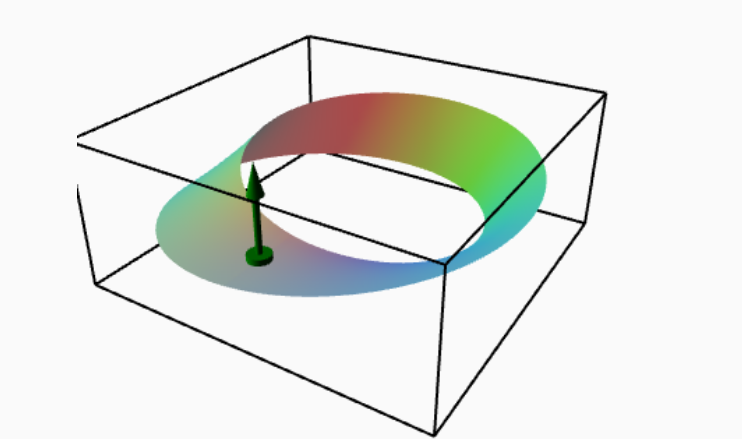
\includegraphics[width=.4\textwidth]{m1.png}
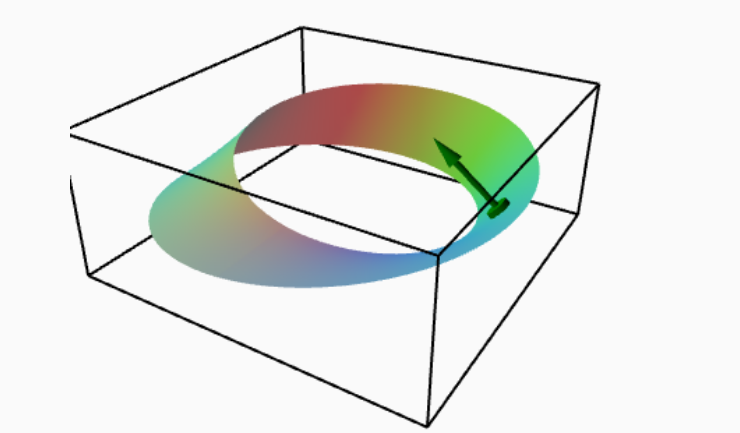
\includegraphics[width=.4\textwidth]{m2.png}
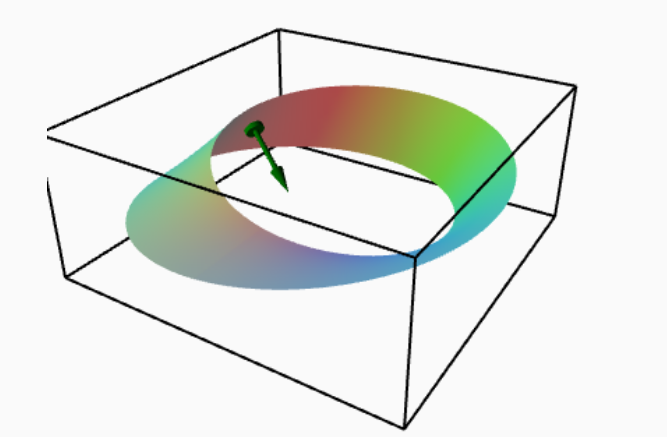
\includegraphics[width=.4\textwidth]{m3.png}
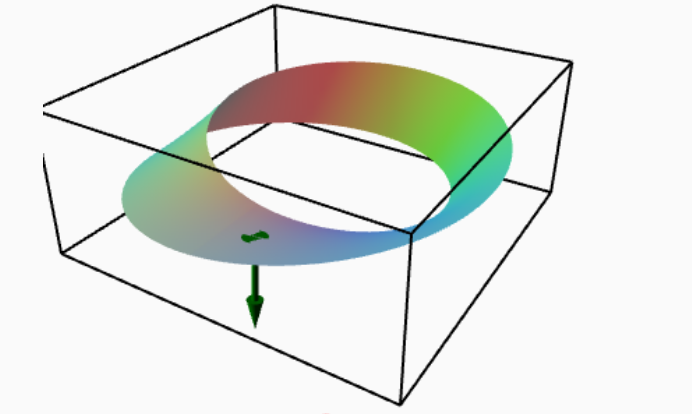
\includegraphics[width=.4\textwidth]{m4.png}
\end{center}

\subsection{Orientable Manifolds} 
Our goal is to express the number of loops in a Reeb graph by the number of critical points. Let $n_i$ be the number of nodes with a degree $i$. Orientable manifolds have zero critical points of degree two because every point is either minimum, maximum or saddle.\\
Therefore the number of arcs is number of connections each point has, divided by two (because we count each arc twice) is $e = (n_1+3n_3)/2$ \\ 
Next, we show that the number of loops is $1+e-(n_1+n_3)$, or in more general case $l=(1+e-v)$ where v is the number of vertices, and l the number of loops
\begin{proof}
    For l = 1, v = 2 and e = 2 so the formula $1=1+2-2$ holds
    \\ Assume that for l = k formula holds \\
    l = (k+1)-loop graph is produced from k-loop graph by either drawing one additional edge between two already existing vertices, which doesn't change $l-e$, or by adding a new vertex and connecting it to two other vertices, which doesn't change $l-i+v$.\\
    By induction, the formula holds.
\end{proof}

\begin{definition}
    Let P be a polyhedron with V vertices, E edges, and F faces. Then we define the Euler characteristic to be 
    \begin{equation}
        \chi(P) = V - E + F  
    \end{equation}
\end{definition} 
More generally, Euler characteristic is defined as an alternating sum of Betti numbers. Last Morse inequality allow us to define $\chi$ as a set of inequalities for alternating sums of Betti numbers in terms of a corresponding alternating sum of the number of critical point $n_i$ of a Morse function of a given index. Namely, let $n$ be the maximum index of all critical points.
\begin{equation}
    \sum_{i=0}^{n} 0 ^n (-1)^i n_i = \chi(P)
\end{equation}
\begin{definition}
    The genus is the maximum number of pairwise disjoint simple closed curves along which we can cut while keeping the manifold in once piece.
\end{definition}
For orientable case we have $ g = (2 - \chi)/2$ and for non-orientable case \\ $ g = 2- \chi$ \\
A connected orientable 2-manifold is either diffeomorphic to the sphere or the connected sum of tori. It's genus is equal to the number of connected tori in diffemorphic image of the manifold.

Let's introduce some concepts that will allow us to prove the following lemma
\begin{definition}[Homotopy]
    A homotopy between two continuous functions $f$ and $g$ from a topological space $X$ to a topological space $Y$ is defined to be a continuous function $H: X \times [0,1] \to Y$ such that $H(x,0) = f(x)$ and $H(x,1) = g(x) \forall x \in X$
\end{definition}
We want to prove that a function $f$ taking a surface to it's Reeb graph is homotopic to the function $g$ taking a surface to it's Reeb graph and removing all the nodes of degree 1. A function is homotopic if an only if it preserves $\chi = v - e$. If we collapse all the nodes of degree 1 in the Reeb graph, for each node we remove 1 edge, therefore $\chi = v - e$ stays constant and $f$ and $g$ are homotopic. \\
Similarly, we prove that a function $f$ is also homotopic to a function $h$ that merges edges across degree 2 nodes which also get eliminated in the process. Again, when we merge two edges, our total number of edges decrease by one, and we collapse the degree 2 node. Thus, $\chi = v-e$ stays the same and $f \sim g$
\begin{lemma}
    The Reeb graph of a Morse function on a connected, orientable 2-manifold of genus g has g loops.
    \begin{proof}
        We first suppose that Reeb graph has no loops. It has $n_1 = n_3+2$. And if we write $c_i$ for the number of critical points of index $i$ we have $n_i = c_0+c_2$ and $n_3 = c_1$. we have $\chi = c_1 - c_1 +c_2 = n_1 - n_3 = 2.$  Where 2 is the Euler characteristic of a sphere, which has no genus. \\ 
        Now suppose that Reeb graph has at least one loop. We can apply following two functions because they preserve homotopy type and the number of loops: collapse degree 1 nodes and merge arcs across degree 2 nodes which get eliminated in the process. For example consider the following graph of double torus:
    \begin{center}

        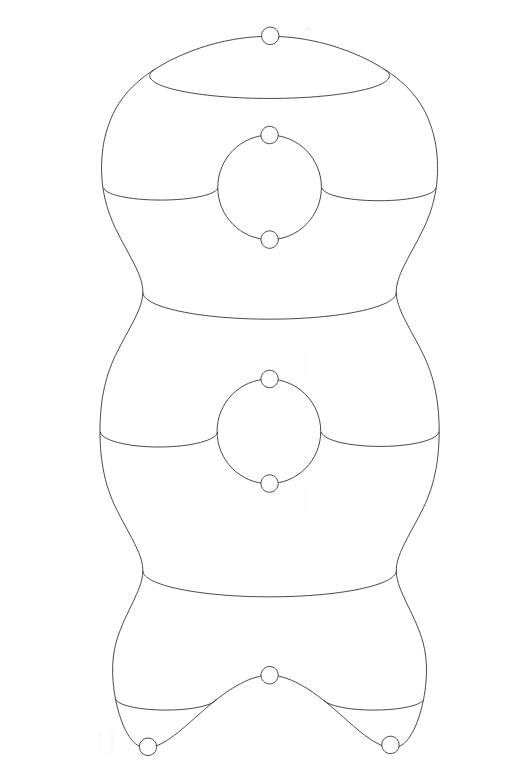
\includegraphics[width=.2\textwidth]{2-tori.png}
        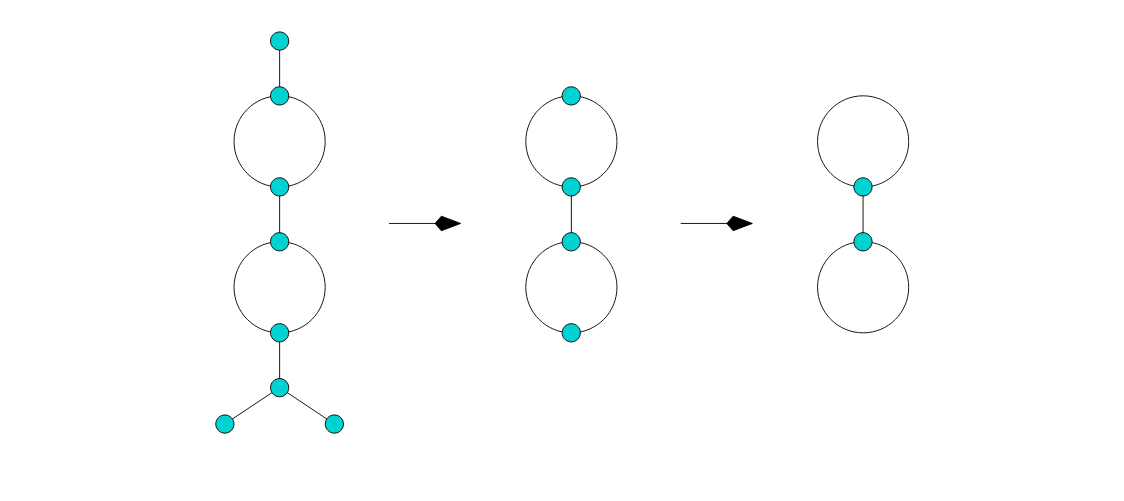
\includegraphics[width=.7\textwidth]{homotopic_transformation.png}
    \end{center}
    Let $m_3$ be the number of remaining degree 3 nodes and note that it is even because $3m_3$ is twice the number of remaining arcs. Using the Euler-Poincare Theorem for graphs we get $\chi = m_3 - 3m_3/2 = \beta_0 - \beta_1$. The graph is connected which implies that the number of loops is $\beta_1 = m_3/2+1$. We have $c_1$ degree 3 nodes in the original Reeb graph and for each minimum and maximum we collapse one degree 1 node removing a 3 degree node in the process. Last strong Morse inequality tells us that $m_3 = c_1 - (c_0 + c_2) = -\chi = 2g - 2$. The number of loops is therefore $ \beta_1 = (2g-2)/2+1=g$
    \end{proof}
\end{lemma}

% % end M2
%%%%%%%%%%%%%%%%%%%%%%%%%%%%%%%%%%%%%%%%%%%%%%%%%%%%%%%%%%%%%%%%%%%%%%%%%%%%%%%%%%%%%%%%%%%%%%%%%%%%%%%%%%%%%%%%%%%%%%%%%%%%%%%%%%%%%%%%%%%%%%%%%%%%%%%%%%%%%%%%%%
%%%%%%%%%%%%%%%%%%%%%%%%%%%%%%%%%%%%%%%%%%%%%%%%%%%%%%%%%%%%%%%%%%%%%%%%%%%%%%%%%%%%%%%%%%%%%%%%%%%%%%%%%%%%%%%%%%%%%%%%%%%%%%%%%%%%%%%%%%%%%%%%%%%%%%%%%%%%%%%%%%
% % begin V2
% % end V2
%%%%%%%%%%%%%%%%%%%%%%%%%%%%%%%%%%%%%%%%%%%%%%%%%%%%%%%%%%%%%%%%%%%%%%%%%%%%%%%%%%%%%%%%%%%%%%%%%%%%%%%%%%%%%%%%%%%%%%%%%%%%%%%%%%%%%%%%%%%%%%%%%%%%%%%%%%%%%%%%%%

% \caption{ 4 figures}

\subsection{Non-orientable 2-manifolds without boundary}

We will consider in this section Reeb graphs of Morse functions over non-orientable 2-manifolds with boundary. In particular, number of nodes, contours and loops in such graphs. \\
All connected non-orientable 2-manifolds without boundary could be expressed as connected sum of  $g$ copies of projective planes $N=P\# P...\# P$, where $g$ coincides with the genus of the surface.\\
For the further proofs we have to recall that Euler characteristic of orientable surfaces can be calculated as $\chi=2-2g$ and for non-orientable it is $\chi=2-g$. Also we have to notice that we can make a 2-sheeted cover of a non-orientable 2-manifold, where each sheet is orientable. In future we will call this $doubling$. \\
Let's consider the process of doubling. We obtain 2-sheeted cover of $N$ (non-orientable 2-manifold) by doubling each point $x\in N$ to two points $x'$ and $x''$. We can consider them as a points lying in the neighborhood of $x$ on two opposite sides of $N$. Union of such points $x'$ and $x''$ will be space that is connected and orientable 2-manifold $M$. Due to the doubling Euler characteristic of the surface will be doubled, $\chi_M=2\chi_N$. \\
Now we have to calculate genus of $M$. Since it is orientable:\\ $g_M=\frac{2-\chi_M}{2}=1-\frac{\chi_M}{2}=1-\chi_N=1-(2-g_N-1)=g_N-1$. \\
Therefore, by doubling we decrease genus by 1. \\
In the table on the fig. \ref{fig:Table} one can find Euler characteristicand genus number of basic non-orianatble manifolds. Note that $K$ is a Klein bottle, $T$ represents torrus,$S$ sphere and $P$ is a projective plane. 
\begin{figure}[h!]
\center{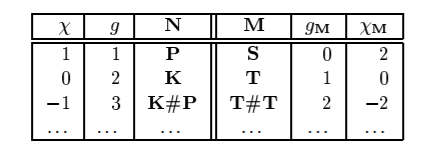
\includegraphics[scale=0.9]{char_table.png}}
\caption{Euler characteristic and genus of some non-orientable manifolds and their doublings}
\label{fig:Table}
\end{figure}
On the table fig. \ref{fig:Table} one can observe that relation of Euler characteristic and genus number of non-orientable manifolds and their doublings coincides with the dependence introduced above. \\
Now we can move on to describing Reeb graphs of non-orientable 2-manifolds without boundary. As an example let's consider Klein bottle, its Reeb graph, and Reeb graph of its doubling surface on fig.\ref{fig:Klein}. \\
\begin{figure}[h!]
\center{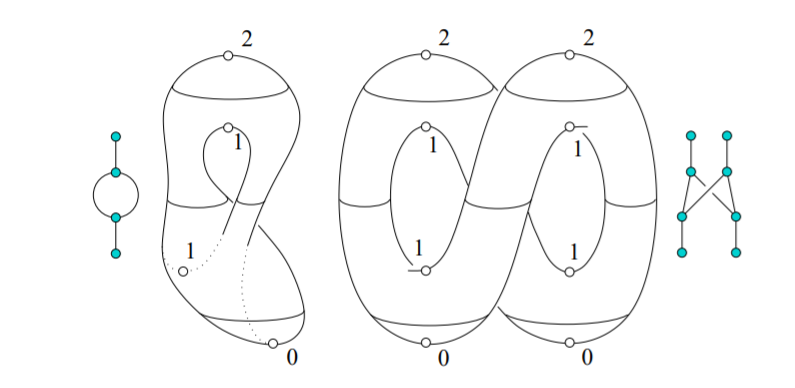
\includegraphics[scale=0.45]{Klein_bottle.png}}
\caption{Reeb graph of Klein bottle and its doubling}
\label{fig:Klein}
\end{figure}
As we see on the fig. \ref{fig:Klein} Reeb graph of the surface drastically changes after doubling, especially number of nodes and contours.  Let's learn how do nodes of each degree change under this doubling. \\
1-degree nodes are maxima or minima, after doubling number of these nodes is doubled and also number of contours is doubled as well. \\
2-degree nodes exist in Reeb graphs of non-orientable surfaces, despite the fact that in orientable surfaces they could be just collapsed. It is transformed into 4-degree node after doubling. The reason is that the level set containing a critical point of index 1 is a figure-8 which may contain an orientation-reversing cycle. \\
3-degree nodes are saddle points that just transfer into two such nodes in its doubling. \\
One could observe the above on the fig. \ref{fig:Nodes}.  
\begin{figure}[h!]
\center{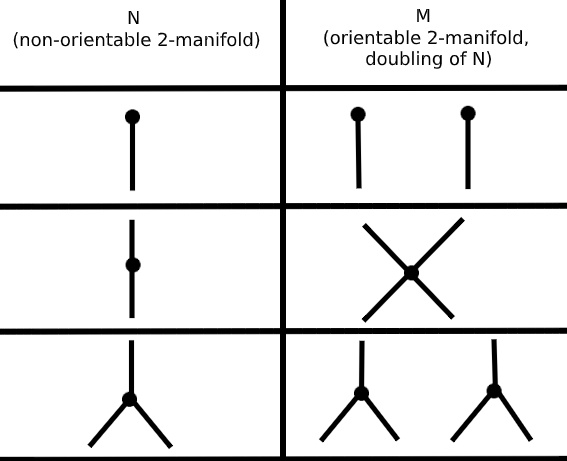
\includegraphics[scale=0.3]{Nodes.png}}
\caption{Correspondence between nodes in $N$ and its doubling $M$}
\label{fig:Nodes}
\end{figure}
Let $f: N \rightarrow R$ is a Morse function that induces function $f_0: M \rightarrow R$. $f_0$ is not a Morse function, since all critical points of $f$ correspond to two critical points of $f_0$, so they are not distinct. However, critical points of $f_0$ are still non-degenerate, that gives as an opportunity to consider $R(f_0)$ (Reeb graph of $f_0$) as previously. \\
Let $e$ be number of arcs in $R(f)$, $n_{1,3}$ is number of 1-degree and 3-degree nodes of $R(f)$, and $n_2$ is number 2-degree nodes. As seen previously, number of 1,3-degree nodes and their contours are doubled in $M$. However, number of 2-degree nodes is invariant under doubling, corresponding contours are doubled. \\
Therefore, $R(f_0)$ has $2e$ arcs and $2n_{1,3}+n_2$ nodes. Known fact that number of loops in a graph is $\beta_1 (G)=1-+e-n$, where $e$ is number of edges(arcs) and $n$ is number of nodes. \\
After substitution we get:\\
$1-\beta_1(R(f_0)=2n_{1,2}+n_2-2e=2-2+2n_{1,3}+2n_2+2e-n_2=2-2(1-n_{1,3}-n_2+e)-n_2=2-2\beta_1(R(f))-n_2$. \\
Also we know that number of loops of $N$ is its genus and genus of $M$ (number of loops) is one less that one of $N$. Therefore, we can make a substitution $\beta_1(R(f_0))=g_N-1$. \\
From the above results we get: \\
$\beta_1(R(f))=\frac{g_N-n_2}{2}$.\\
Since number of 2-degree nodes $n_2\geq0 $, we may obtain the following result:\\
\begin{lemma}
The Reeb graph of a Morse function over connected non-orientable 2-manifolds of genus $g$ with boundary is at most $\frac{g}{2}$.\\
\end{lemma}

\section{Applications}
\subsection{Topological Data Analysis}
A computational method for extracting simple descriptions of high dimensional data sets is a Mapper algorithm:
Let $X$ be a point cloud (data set) and we have a function $f:X \to \R$.
Assume that we have $N$ points in $X$ whose outputs are known for the function $f$.
Also, we assume that it is possible to compute inter-point distances between the points in the data.
Let $I$ be the range of the function $f$ restricted to the $N$ points and let $S$ be the covering of $I$.
We begin by dividing $S$ into a smaller intervals $(S_i)$ which overlap.
This gives us two parameters $l_i$ the length of $S_i$ and $p_{ij}$ the perceptange overlap between successive intervals.
Now for each $S_i$ we find a set $X_j = \{x | f(x) \in S_j\}$ s.t. $X_j \subset X$. The set $\{X_j\}$ forms a cover of $X$, and $X \subset \cup_j X_j$.
For each smaller set $X_j$ we find clusters $\{X_{jk}\} $.
We treat each cluster as a vertex in our reeb graph and draw an edge between vertices whenever $X_{jk} \cap X_{lm} \neq \emptyset$ i.e. the clusters corresponding to vertices have non-empty intersection. \\


\textbf{Ex.} Find a Reeb graph of a point cloud that has a shape of torus under the function $f(x,y,z) = z$. Approach the problem with assumption that we don't know the underlying distribution i.e. we don't know that it is a shape of torus. \\
Consider the following picture
\begin{center}
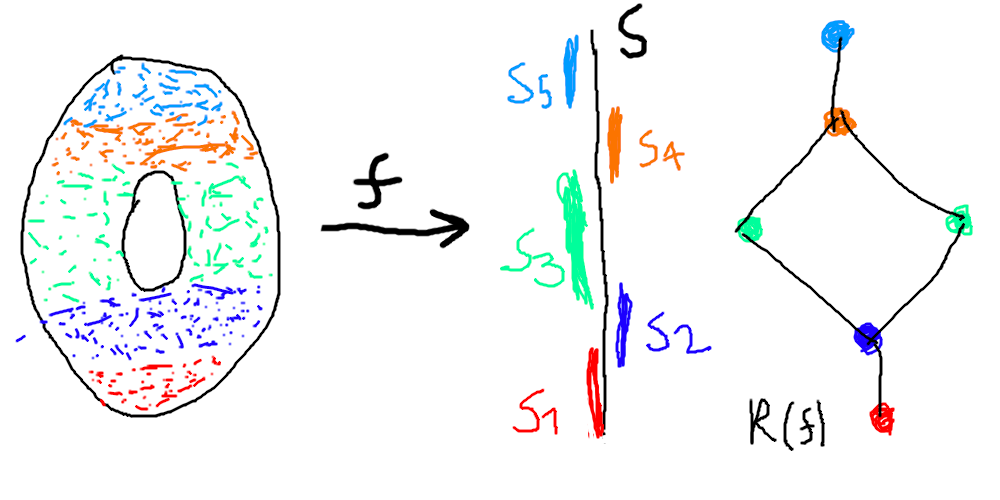
\includegraphics[width=1.0\textwidth]{mapper.png}
\end{center}
We have a map $f:N\to \R$ where N is a set of points in shape of torus.
We create a covering $S$ of the image $f(N)$ and we split the covering into 5 small overlaping intervals.
Now we consider $X_i = f^{-1}(S_i)$ and apply clustering algorithm on the output of the function.
For $X_1$, $X_2$, $X_4$ and $X_5$ there is only one cluster so we draw one vertex, but for $X_3$ we draw two.
Now we check that following clusters overlap: $X_{11} \cap X_{21} \neq \emptyset $, $X_{21} \cap X_{31} \neq \emptyset $, $X_{21} \cap X_{32} \neq \emptyset $, $X_{31} \cap X_{41} \neq \emptyset $,$X_{32} \cap X_{41} \neq \emptyset $,$X_{32} \cap X_{41} \neq \emptyset $.So there's a connection between vertices that represent those clusters. The output is a Reeb graph. \\ 
A famous example of application of Mapper algorithm is implemented by Nikolau, Levine and Carlsson in Topology based data analysis. They are able to identify a subgroup of breast cancers with a unique mutational profile and excellent survival.\\

We have implemented the Mapper algorithm in python and ran it for the sklearn diabetes dataset and standford cars dataset, output are as follows:

\begin{center}
    diabetes 
    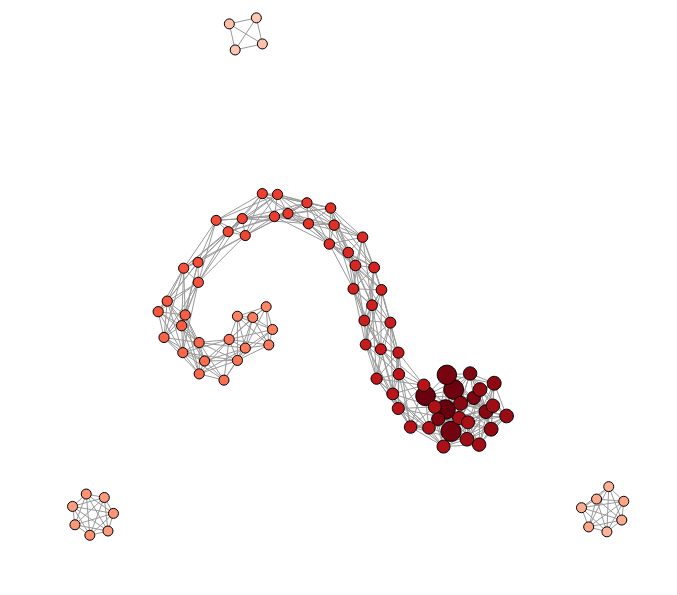
\includegraphics[width=.4\textwidth]{diabetes.png} 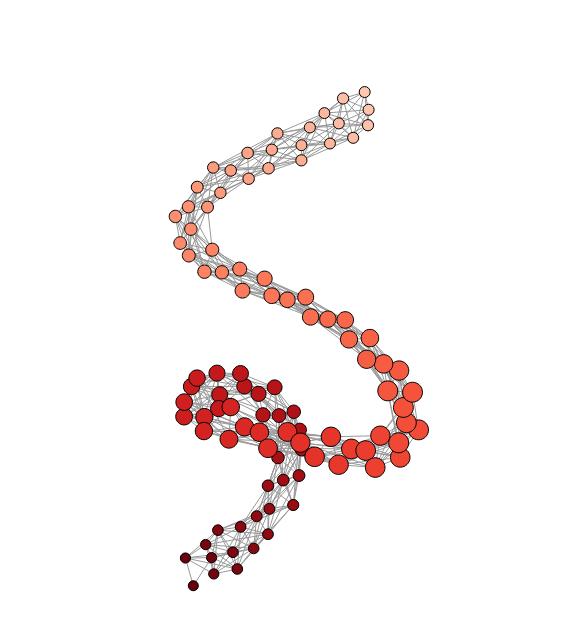
\includegraphics[width=.4\textwidth]{cars.png}
    cars
\end{center}
Based on the diabetes data we may be able to make a difference between patients who don't need a treatmant, patients with diabetis type 1 and patients with diabetis type 2. While in the cars dataset it looks like there aren't any great differences between car features. (the graph is connected)

\subsection{Computer Graphics}
Computer graphics, in particular 3D modeling and animation, are a vast field. Building 3D models and analyzing their features are important both in entertainment (cartoons, animated films, computer games) and for scientific research (building 3D models based on photographs of a microscope for biology and medicine; building physical interactions in mechanics, astronomy, atomic physics ). There are two problems associated with 3D modeling, which are solved using Reeb graphs.\\

 First of all, this is the construction of skeletons of already existing 3D models. This is important for further animation of objects. As shown above, using computer algorithms, we can construct a Reeb graph for any surface. Roughly speaking, this will be the skeleton of our figure. Previously, contour trees were used for these tasks, but this method results in a lot of artifacts, and is not applicable to more complex topological objects. With the help of Reeb graphs simplification algorithms (collapsing second-degree vertices, combining some edges), we can improve the skeleton without losing topological properties. This will optimize further work with the model fig. \ref{fig:skeleton}.

\begin{figure}[h!]
\center{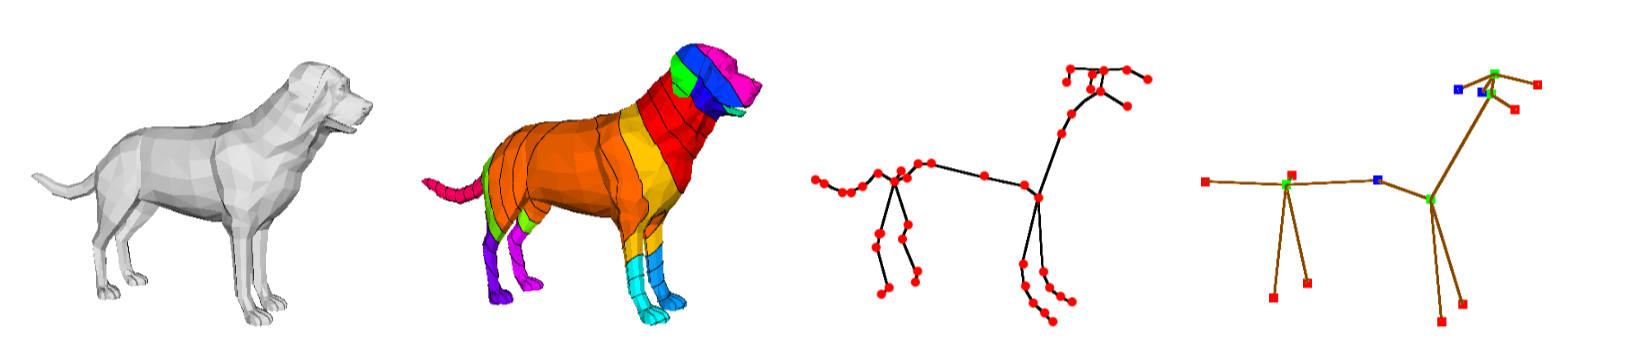
\includegraphics[scale=0.3]{skeleton.png}}
\caption{Skeleton of the model as a Reeb graph and its simplification}
\label{fig:skeleton}
\end{figure}

The second problem of 3D modeling is to simplify mesh triangulation of models. Having a video of some object (or a photo from different angles), common algorithms easily triangulate it. However, this triangulation is often over-fitting. The most common simplification algorithm is the Quadric error method. If the vertex is at a small distance from the plane drawn through its neighbors, then the vertex is removed. Despite the simplicity of this method, it gives a miss-simplification fig. \ref{fig:QED}.\\
\begin{figure}[h!]
\center{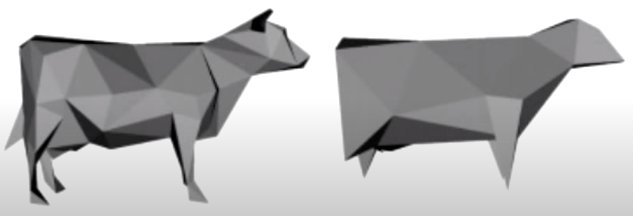
\includegraphics[scale=0.6]{QEM.png}}
\caption{Miss-simplification of QED method}
\label{fig:QED}
\end{figure}

The new method uses Reeb graphs to simplify triangulation. This allows us to save the topological properties of the model after simplification. The idea of the algorithm is to remove those vertices whose geodesic distance to the vertices of the Reeb graph of the model is the smallest. This way we get a more accurate triangulation, with fewer edges. Thanks to the use of the Reeb graphs, all topological properties are preserved in the construction fig. \ref{fig:New_alg}.
\begin{figure}[h!]
\center{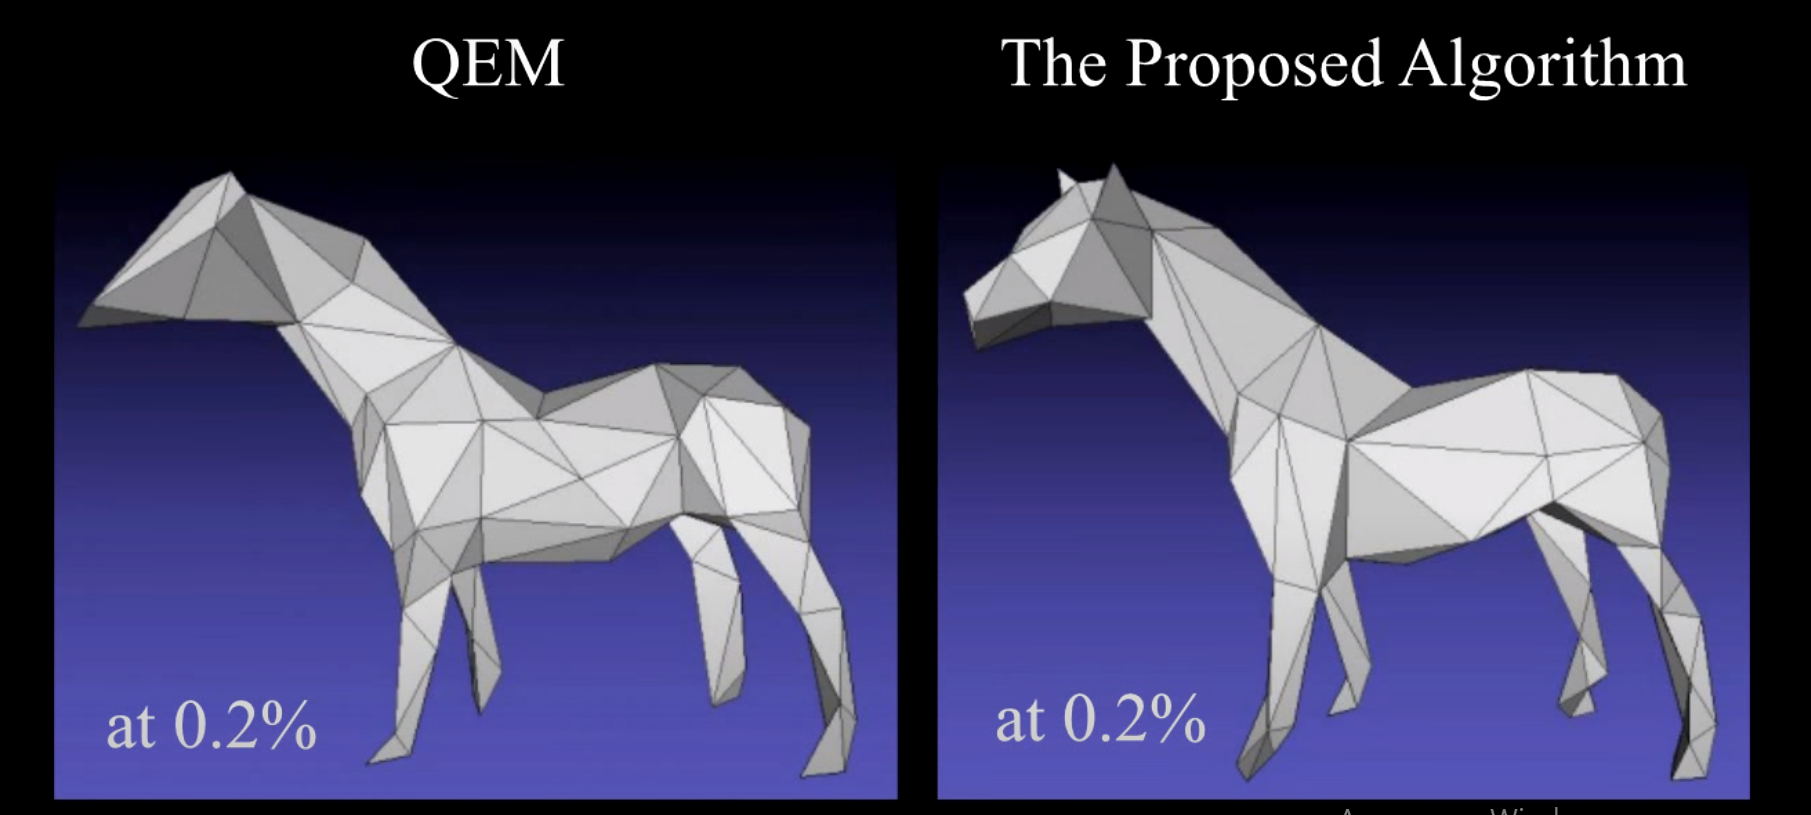
\includegraphics[scale=0.3]{New_alg.png}}
\caption{Comparison of QEM method and the mew algorithm using Reeb graphs}
\label{fig:New_alg}
\end{figure}
\subsection{Oceanography}
    Reeb graphs are used in Oceanography to analyze the flows in the deep ocean. The neutral density $\gamma^n$ is a density variable that is used 
    for describing the so called neutral density surfaces which are aligned with the neutral tangent plane. The flows in the deep ocean are believed to be aligned with the neutral
    tangent plane.

    A neutral surface is a surface that is everywhere parallel to the neutral tangent plane. It is proved that this plane and all neutral surfaces are normal to
    the dianeutral vector:
   $$
    \vec{N}=\rho(\beta \nabla S-\alpha \nabla\theta)
   $$

   where $S$ is the salinity, $\theta$ is the potential temperature, $\alpha$ is the thermal expansion coefficient,
   and $\beta$ is the saline concentration coefficient. Therefore, neutral surfaces are perpendicular to $\vec{N}$ in every point. It is proved that:

   The neutral density is a function of latitude and longitude. The spatial dependence is fundamental property
   of neutral surfaces. Since the gradients of $S$ and $\theta$ within a neutral surface are aligned, their contours are also aligned.
   Therefore, there is a functional relationship between these variables. It is proved that the regions where
   the function is single-valued are the regions associated with the edges of the Reeb graph of $\theta$ on the surface.

\begin{thebibliography}{9}
     \bibitem{MorseTheory}
     {\sc Hua Amy}
       An introductory treatment of morse theory on manifolds
       \href{http://www.math.uchicago.edu/~may/VIGRE/VIGRE2010/REUPapers/Hua.pdf}{http://www.math.uchicago.edu/~may/VIGRE/VIGRE2010/REUPapers/Hua.pdf}
     \bibitem{Reebgraphs}
     {\sc Cole-McLaughlin at al.} 
       `` Loops in Reeb Graphs of 2-Manifolds  \href{https://core.ac.uk/download/pdf/20670562.pdf}{https://core.ac.uk/download/pdf/20670562.pdf}
     \bibitem{Mapper}
         {\sc Singh at al. }
          Loops in Reeb Graphs of 2-Manifolds \href{http://www.math.uchicago.edu/~may/VIGRE/VIGRE2010/REUPapers/Hua.pdf}{http://www.math.uchicago.edu/~may/VIGRE/VIGRE2010/REUPapers/Hua.pdf}
    \bibitem{Textbook}
        {\sc Allan Pollack and Victor Guillemin } 
        Differential Topology
\end{thebibliography}
\end{document}
